\label{sec:5.4}

%%%%%%%%%%%%%%%%%%%%%%%%%%%%%%%%%%%%%%%%%%%%%%%%%%%%%%%
%(Prakash) Discuss SHA/MUX linearity
%%%%%%%%%%%%%%%%%%%%%%%%%%%%%%%%%%%%%%%%%%%%%%%%%%%%%%%

The input signals are sampled at a rate of 2 MS/s, multiplexed by 8 and digitized by one of two calibrated 12-bit pipelined ADCs operating at 16 MS/s. The linearity of the ADC to a small extent depends on the linearity of the SHA/MUX circuit aswell. 

ColdADC can be calibrated to an amazing degree. The ability to configure and isolate the MUX's turned out to be very helpful to lock down the linearity issue. The linearity of the ADC is approximately reduced by 0.3 LSB when SHA is in free running mode (MUX is operating). Figures \ref{fig:linearity_freesha} and \ref{fig:linearity_frozensha} show the difference in linearity for free running and frozen SHA. 

\begin{figure}[h!]
\centering
  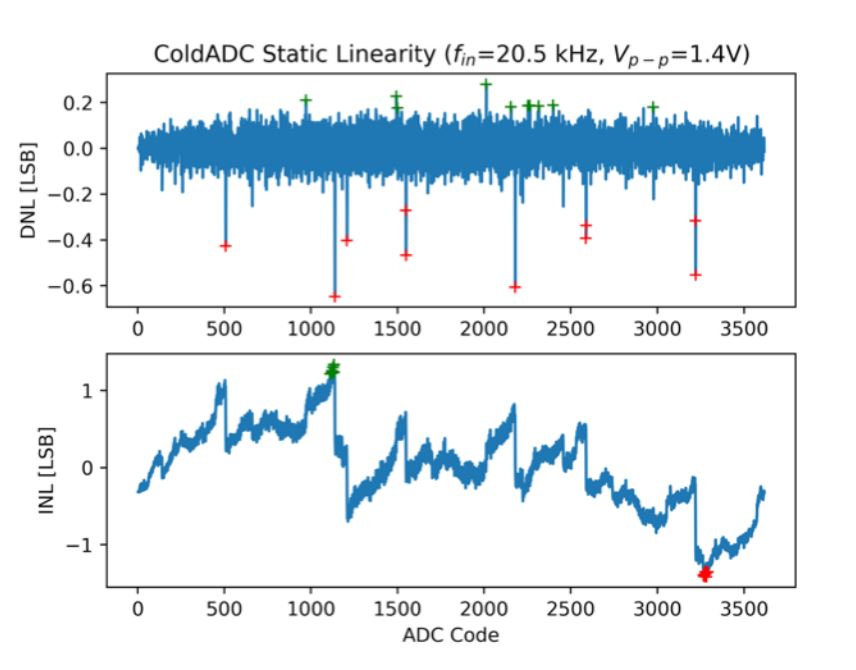
\includegraphics[width=0.7\linewidth]{figures/prakash_fig/linearity_freesha.JPG}
  \caption{}
  \label{fig:linearity_freesha}
\end{figure}

\begin{figure}[h!]
\centering
  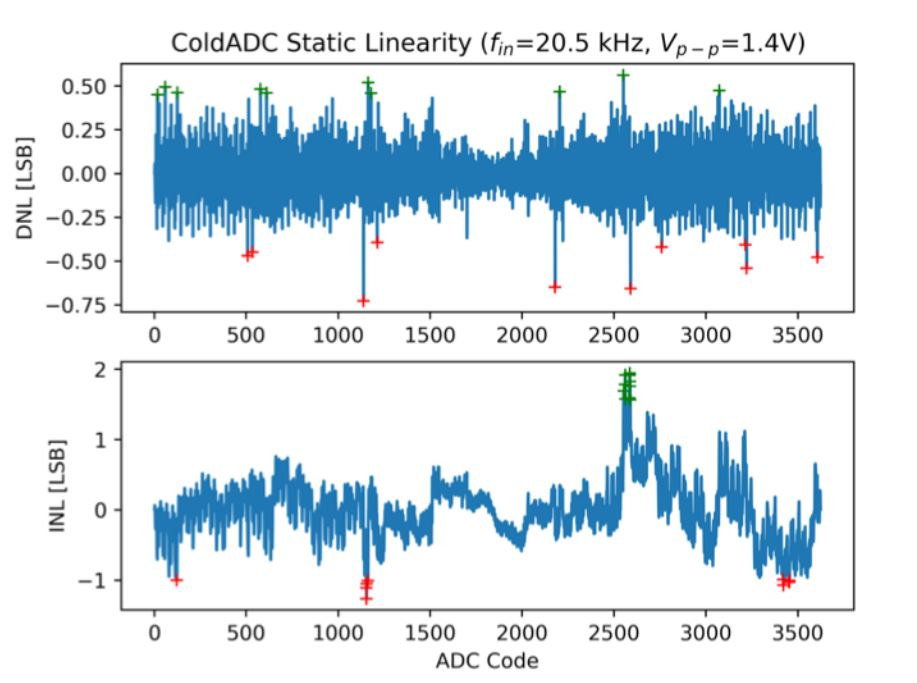
\includegraphics[width=0.7\linewidth]{figures/prakash_fig/linearity_frozensha.JPG}
  \caption{}
  \label{fig:linearity_frozensha}
\end{figure}

Evidence of linearity degradation only during the free running SHA mode indicate two possible issues, possible overlapping of the clocks for the MUX's and/or insufficient settling of MUX's. It is very difficult to simulate MUX's effects on ADC linearity. We are still looking to understand the root cause for linearity degradation. To improve this we will redesign the MUX's to be faster and improve the clocking scheme. 